La visión nocturna se crea tomando luz en el espectro infrarrojo y amplificándola, haciendola más brillante. La longitud de onda de esta luz se encuentra aproximadamente entre los 750 nm y 1400 nm. A los dispositivos que emplean visión nocturna se les conoce con las siglas \textbf{NVD} (\textit{Night Vision Device}). Para uso militar son muy comunes las gafas de visión nocturna o \textbf{NVG} (\textit{Night Vision Google}), por ejemplo la \textbf{GPNVG} (\textit{Ground Panoramic Night Vision Google}), que ofrece un mayor campo de visión al combinar 4 lentes.

\begin{figure}[H]
  \centering
  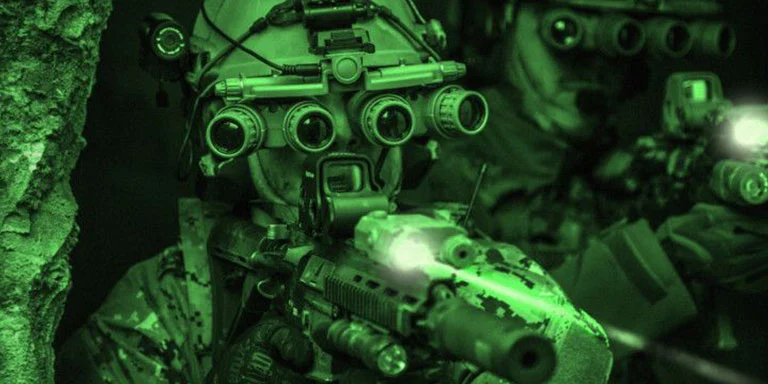
\includegraphics[scale=0.4]{imagenes/nvg.png}
  \caption{GPNVG\cite{tactgearnv}}
\end{figure}

La imagen se genera a trvés de una pantalla de fósforo. Durante décadas ha sido verde. Sin embargo, en condiciones oscuras el ojo humano no ve mejor en la parte verde del espectro. Los fotoreceptores en la retina especializados para la visión con poca luz tienen su pico de sensibilidad en la parte azul de espectro. Para lograr una mejor visión se usa una pantalla de fósforo blanco, que se ve azul claro.

\subsection{Procedimiento}

\begin{figure}[H]
  \centering
  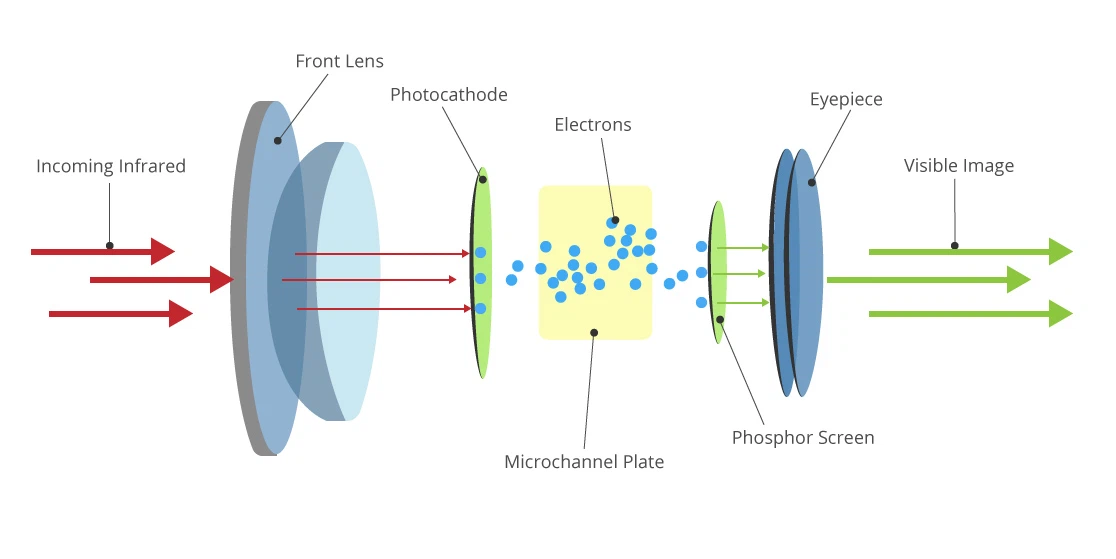
\includegraphics[scale=0.4]{imagenes/vision_nocturna.png}
  \caption{Proceso de generar visión nocturna\cite{jpnvnv}}
\end{figure}

En un lugar oscuro debe haber alguna fuente de energía, por ejemplo luz visible de las estrellas o calor de un cuerpo, que es recibida por un \textbf{tubo de intensificación de imagen}. Una lente enfoca los fotones dentro del tubo como una imagen al revés donde, pasan por tres pasos.

En primer lugar el fotón golpea una placa fina llamada \textbf{fotocátodo} (\textit{Photocathode}), hecha de semiconducores o metales alcalinos, en un punto. Un electrón en ese punto de la placa es excitado y es ejectado en un espacio vacío. Los electrones son acelerados a través del tubo de vacío por un voltaje, por ejemplo 800 V.

En segundo lugar los electrones se dirigen hacia otra placa fina llamada \textbf{placa microcanal} (\textit{Microchannel Plate}). Esta placa está hecha de un material aislante, generalmente vidrio, y cuenta con aproximadamente 6 millones de canales muy pequeños. Estos canales tienen un ángulo de 5 grados en sentido horario, con el objetivo de que los electrones entrantes colisionen con las paredes de los canales. Al hacer esto se crean más electrones de la pared del material, que colisionan con las paredes y crean aun más electrones. Por lo tanto, entran unos pocos y salen miles. Estos electrones salen de los canales y vuelven a ser acelerados en linea recta por otro voltaje más alto, por ejemplo 5800 V.

En tercer lugar los miles de electrones golpean una \textbf{pantalla de fósforo} (\textit{Phosphor Screen}). Esta es una pantalla hecha de material que brilla cuando se expone a la radiación. Por los tanto, convierte la energía cinética de los electrones de vuelta a fotones visibles para el ojo humano.

Cada fotón que entra en el tubo es multiplicado miles de veces manteniendo su posición, lo cual genera una imagen más brillante e identica. Como último paso, hay millones de fibras ópticas, por ejemplo 20 millones, ligadas a la pantalla de fósforo que giran la imagen hacia arriba\cite{ytvrtbv}.

\subsection{Tipos}

\begin{figure}[H]
  \centering
  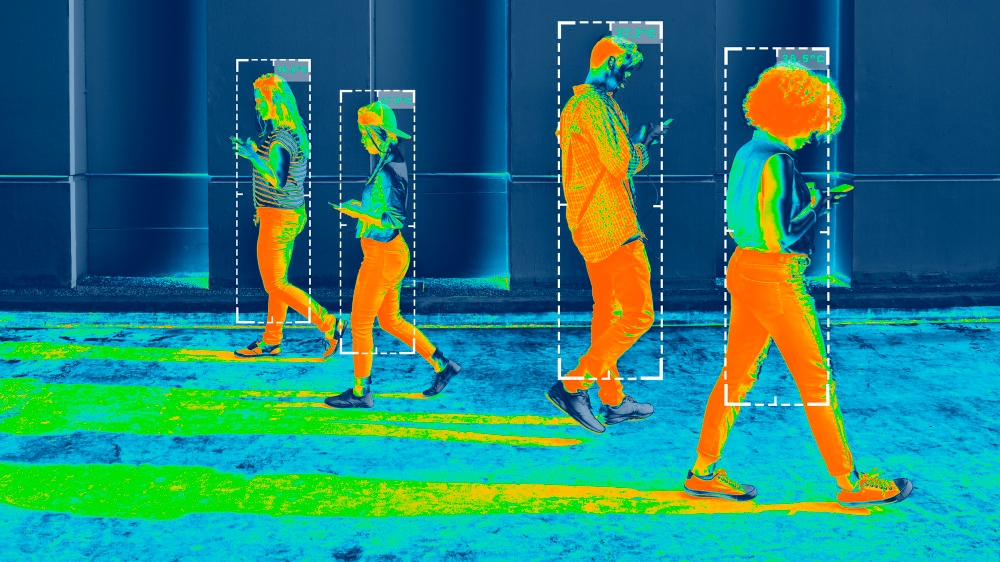
\includegraphics[scale=0.3]{imagenes/imagen_termica.png}
  \caption{Imagen térmica\cite{bytronicti}}
\end{figure}

\textbf{Iluminación Activa} (\textit{Active Illumination}): crean su propia luz, como la de una linterna. Es la más fácil de producir y es la común para uso general, como cámaras de seguridad. El color de la imagen es blanco y negro.

\textbf{Intsensificación de Imagen} (\textit{Image Intensification}): amplifica luz existente. Se utiliza mucho en el ejército. El color de la imagen depende de la lente de fósforo, verde o azul claro.

\textbf{Imagen Térmica} (\textit{Thermal Imaging}): crea imágenes a partir de bandas de emisión infrarroja. Cámaras térmicas de alta calidad son muy grandes y consumen mucha energía para ser portables.. El color de la imagen depende de la intensidad de la fuente de emisión, colores fríos o cálidos.
